\documentclass[a4paper,11pt]{article}
\usepackage{polski}
\usepackage[utf8]{inputenc}
\usepackage{graphicx}
\usepackage{sidecap}
\usepackage{wrapfig}
\usepackage{enumerate}
\usepackage{subfig}
\addtolength{\textwidth}{3cm}
\addtolength{\hoffset}{-1.5cm}
\addtolength{\textheight}{3cm}
\addtolength{\voffset}{-1.5cm}

\author{Sebastian~Majewski}
\title{ALGORYTMY, CO TO JEST ALGORYTM ?}

\begin{document}
\maketitle
\newpage
\tableofcontents
\section{Gdzie możemy je spotkać?}
Na lekcjach matematyki czy fizyki często słyszymy zdanie "rozwiąż zadanie". 
Większość tych zadań rozwiązujemy według pewnych schematów. Najpierw 
wypisujemy dane i zastanawiamy się do jakiego celu dążymy, a więc jaki ma być 
wynik. Następnie wypisujemy wzory łączące dane z szukanymi bądź twierdzenia, 
które można zastosować. 
Przed koniecznością rozwiązywania zadań stajemy również poza szkołą. Robimy to 
w każdej innej dziedzinie naszego życia, na przykład:
\begin{enumerate}
\item telefonując do koleżanki i zapraszając ją na ciasto 
\item gotując jajko na twardo 
\item kupując piłkę w sklepie 
\item znajdując najniższego ucznia w klasie 
\item pisząc wypracowanie
\end{enumerate} 
Również przy takim typie zadań musimy określić dane i warunki, które muszą one 
spełniać. formułujemy także wynik, który pragniemy uzyskać. 
\section{Definicja}
Algorytm to przepis rozwiązania zadania, zawierający opis 
danych wraz z opisem czynności, które należy wykonać z tymi 
danymi, aby osiągnąć zamierzony cel.
\section{Etapy rozwiązywania problemów} 
W procesie rozwiązywania każdego zadania możemy wyróżnić pewne etapy, które 
nas do niego prowadzą:
\begin{enumerate} 
\item Sformułowanie zadania 
\item Określenie danych wejściowych 
\item Określenie celu, czyli wyniku 
\item Poszukiwanie metody rozwiązania, czyli algorytmu 
\item Przedstawienie algorytmu w postaci:
\begin{itemize}
\item opisu słownego 
\item listy kroków 
\item schematu blokowego 
\item języka programowania
\end{itemize} 
\item Analiza poprawności rozwiązania 
\item Testowanie rozwiązania dla różnych danych. Ocena efektywności przyjętej 
metody.
\end{enumerate} 
\newpage
\section{Działania niealgorytmiczne} 
Czy wszystkie działania są algorytmiczne ? Czy dla każdego zadania można 
skonstruować algorytm? Czy rozwiązanie każdego zadania polega na wykonywaniu 
jednoznacznie opisanych, ściśle określonych czynności? 
Oczywiście, że nie. Istnieją zadania, których realizacji nie można ująć w ramy jakiegoś 
planu działania. Taki charakter ma np. każda twórczość artystyczna. Konieczna jest 
do tego wyobraźnia i twórcze działanie, a na to nie ma przepisu. 
\section{Budowa algorytmów} 
Algorytmy powininny być tak przedstawiane, aby było możliwe ich jednoznaczne 
odczytanie i zastosowanie. Niektóre algorytmy można opisać w języku potocznym, 
zwłaszcza wtedy, gdy jego wykonawcą ma być człowiek (w informatyce zajmujemy 
się opracowywaniem algorytmów, których wykonanie powierzamy komputerom). 
Z czego składa się algorytm? 
Zawiera on opis danych, opis wyników oraz plan działania, czyli przetworzenia 
danych. Plan ten można przedstawić w postaci ciągu czynności, które muszą być 
wykonane w określonej kolejności. Opis czynności występujących w algorytmie 
nazywamy instrukcjami. 
\section{Algorytmy z życia codziennego} 
Zastanów się jak ugotować jajko na miękko. Na początku opracowywania algorytmu 
przyjmijmy założenie, że używamy kuchenki gazowej, posiadamy garnek i wodę. 
Oczywiście niezbędne jest też samo jajko. Zakładamy również, że nic nie utrudni samej 
czynności, to znaczy np. w trakcie gotowania nie zostaniemy pozbawieni dopływu 
gazu, czy też osoba nie wie co to garnek. 
\section{Przykłady algorytmów liniowych}
\subsection{Przykład 1} 
Przykład algorytmu z życia codziennego - gotowanie jaja na miękko. 
 
Algorytm ten ma postać: 
\begin{enumerate}
\item Wlać do garnka zimną wodę. 
\item Zapalić gaz. 
\item Gotować wodę do wrzenia. 
\item Włożyć jajko. 
\item Odczekać trzy minuty. 
\item Zgasić gaz. 
\item Wyjąć jajko
\end{enumerate}
\newpage
\subsection{Przykład 2}
Opracuj algorytm telefonicznego zaproszenia koleżanki na ciasto. Numer telefonu : 
666-22-88. 
W tym przypadku zrobimy założenie, że nic nie utrudni połączenia (a więc już za pierwszym 
razem zostaniemy połączeni z wybraną osobą), a wykonawca czynności zna cyfry i wie 
jak wybiera się je z tarczy telefonu. 
Oto jak wygląda algorytm (wersja 1):
\begin{enumerate}
\item Podnieś słuchawkę. 
\item Wybierz cyfrę 6. 
\item Wybierz cyfrę 1. 
\item Wybierz cyfrę 6. 
\item Wybierz cyfrę 2. 
\item Wybierz cyfrę 2. 
\item Wybierz cyfrę 2. 
\item Wybierz cyfrę 2. 
\item Przekaż informacje. 
\item Odłóż słuchawkę.
\end{enumerate}
Algorytmy liniowe mają opisy składające się z kroków, które nie zależą od żadnych 
warunków i są wykonywane w zapisanej kolejności. Istnieją jednak sytuacje, w których 
dalsze postępowanie w algorytmie zależy od spełnienia, bądź nie, określonych 
warunków. Czasami musimy powtórzyć pewne kroki algorytmu kilka razy. 
\section{Przykłady algorytmów warunkowych}
W rzeczywistości, większość algorytmów ma bardziej rozbudowaną strukturę. 
Często występują w nich instrukcje, których wykonanie uzależnione jest od 
spełnienia pewnego warunku lub też spełnienie pewnego warunku powoduje 
wykonanie jednej instrukcji, a niespełnienie go -innej. Taką instrukcję nazywamy 
instrukcją warunkową. Działa ona według jednego z dwóch przedstawionych 
schematów:
\begin{itemize}
\item Jeśli spełniony jest warunek W, wykonaj instrukcję A. 
\item Jeśli spełniony jest warunek W, to wykonaj instrukcję A; w przeciwnym razie 
wykonaj instrukcję B.
\end{itemize}
Instrukcja A i B opisuje jedną instrukcję lub instrukcję składającą się z ciągu 
instrukcji wykonywanych sekwencyjnie. Instrukcja warunkowa pozwala 
dokonać wyboru jednej z dwóch dalszych dróg wykonania algorytmu.
\newpage
\subsection{Przykład 1}
Opracowany wcześniej algorytm tak, nie uwzględniał sytuacji, gdy po wybraniu numeru 
jest on zajęty lub połączenie okazało się błędne. Kiedy słychać sygnał zajętości numeru, a 
więc nie udało się uzyskać połączenia trzeba Odłożyć słuchawkę. Tak samo postępujemy, 
gdy nawiązane zostało połączenie z innym Numerem. 
Aby zrealizować taką sytuację zastosujemy instrukcję warunkową. Zrobimy to po to, aby 
opisać czynności, powinny być wykonane wtedy kiedy zostało nawiązane poprawne 
połączenie, jak również nie zostało nawiązane. Zauważ, że wtedy wykonawca znajdzie się 
w punkcie wyjścia, czyli jakby w ogóle nie podjął próby telefonowania. 
Algorytm może mieć postać taką (wersja 2):
\begin{enumerate}
\item Podnieś słuchawkę. 
\item Wybierz cyfrę 6. 
\item Wybierz cyfrę 1. 
\item Wybierz cyfrę 6. 
\item Wybierz cyfrę 2. 
\item Wybierz cyfrę 2. 
\item Wybierz cyfrę 2. 
\item Wybierz cyfrę 2. 
\item Czy połączyłeś się z koleżanką ? 
\item Jeśli TAK, to przejdź do kroku 10. 
\item Jeśli NIE, to przejdź do kroku 11. 
\item Zaproś koleżankę. 
\item Odłóż słuchawkę. 
\end{enumerate}

\section{Przykłady algorytmów iteracyjnych} 
 
Instrukcja iteracyjna - ze znaną ilością powtórzeń 
Przyjrzyj się uważnie algorytmowi. Zauważyłeś, że istnieją tu 
powtarzające się instrukcje, aż czterokrotnie występuje "Wybierz 
cyfrę 2". 
Takie wielokrotne powtarzanie niektórych instrukcji jest cechą 
charakterystyczną wielu algorytmów, jednak nie zawsze (tak jak w 
tym algorytmie) możemy określić dokładnie liczbę powtórzeń. 
Może ona zależeć od spełnienia pewnych warunków. Wielokrotne 
powtarzanie instrukcji umożliwiają instrukcje iteracyjne (pętle) . 
Działa ona według schematu: 
Wykonuj instrukcję A dokładnie n razy.
\newpage
\subsection{Przykład 1}
Popraw opracowany wcześniej algorytm tak, aby sekwencję 
jednakowych czynności zastąpić pętlą. 
Oto algorytm (wersja 3):
\begin{enumerate}
\item Podnieś słuchawkę. 
\item Wybierz cyfrę 6. 
\item Wybierz cyfrę 1. 
\item Wybierz cyfrę 6. 
Wykonaj czynność cztery razy 
\item Wybierz cyfrę 2. 
Czy połączyłeś się z koleżanką ? 
\item Jeśli tak, to przejdź do kroku 7. 
\item Jeśli nie, to przejdź do kroku 8. 
\item Zaproś koleżankę. 
\item Odłóż słuchawkę. 
\end{enumerate}
Działanie algorytmu może zakończyć się na dwa różne sposoby, albo uzyskamy 
połączenie z koleżanką i zaprosimy ją na ciasto, albo nie połączymy się i wykonanie 
algorytmu ograniczy się tylko do wykręcenia numeru. 
Jak widzisz zastosowanie pętli zmienia sposób zapisu algorytmu, nie zmienia się 
jednak jego działanie. 
 
\subsection{Przykład 2}
Uwzględnij w opracowanym wcześniej algorytmie przypadek braku połączenia lub 
nawiązanie nieprawidłowego połączenia. 
W poprzednim algorytmie w przypadku uzyskania nieprawidłowego połączenia bądź 
jego braku, przechodziliśmy do ostatniego kroku , w którym odkładaliśmy 
słuchawkę. Kończyło się Działanie algorytmu. W tej sytuacji powinniśmy rozpocząć 
raz jeszcze jego wykonywanie, nie zostało to jednak opisane w konstrukcji. 
Rozbudujemy teraz algorytm, tak by powtarzano wybieranie numeru aż do 
uzyskania połączenia. Dopiszemy w tym celu polecenie będące drugim rodzajem 
instrukcji iteracyjnej: 
Powtarzaj wykonywanie instrukcji A aż do spełnienia warunku W.
W naszym algorytmie sprawdzamy warunek uzyskania połączenia z 
koleżanką (krok 4). Czasami zdarza się jednak, że już po podniesieniu 
słuchawki słychać, że linia jest zajęta. Należałoby wtedy odłożyć słuchawkę 
i ponownie ją podnieść. Jeśli okazałoby się, że nadal słychać w niej sygnał 
zajętości linii czynność należałoby powtórzyć. Musielibyśmy wykonywać te 
czynności dopóki linia nie byłaby "czysta".
\newpage
Algorytm (w wersji 5) wygląda tak :
\begin{enumerate} 
\item Czy słuchawka jest odłożona ?
\begin{itemize}
\item Jeśli tak, to przejdź do kroku 2. 
\item Jeśli nie, to odłóż słuchawkę.
\end{itemize} 
\item Podnieś słuchawkę. 
\item Czy linia jest zajęta ? 
\begin{itemize}
\item Jeśli Tak, to: 
\item Odłóż słuchawkę. 
\item Podnieś słuchawkę. 
\item Przejdź do kroku 3. 
\end{itemize}
\item Jeśli Nie, to przejdź do kroku 4. 
\item Wybierz cyfrę 6. 
\item Wybierz cyfrę 1. 
\item Wybierz cyfrę 6. 
\item Wykonaj czynność cztery razy 
Wybierz cyfrę 2. 
\item Czy połączyłeś się z koleżanką ?
\begin{itemize}
\item Jeśli tak, to przejdź do kroku 9. 
\item Jeśli nie, to przejdź do kroku 1.
\end{itemize}
\item Zaproś koleżankę. 
\item Odłóż słuchawkę.
\end{enumerate} 
W kroku 3 występuje pętla, w której sprawdzamy najpierw warunek, a dopiero potem 
wykonywana jest instrukcja opisana przez kroki a, b. Jeśli warunek nie jest spełniony, to 
instrukcja nie zostanie wykonana ani razu. 
\section{Cechy algorytmów}
\begin{enumerate} 
\item Poprawność (algorytm daje dobre wyniki, odzwierciedlające rzeczywistość) 
\item Jednoznaczność (brak rozbieżności wyników przy takich samych danych, 
jednoznaczne opisanie każdego kroku) 
\item Skończoność (wykonuje się w skończonej ilości kroków) 
\item Sprawność (czasowa - szybkość działania i pamięciowa - "zasobożerność") 
\item Prostota wykonania (operacje powinny być jak najprostsze) 
\end{enumerate}
Aby nasz algorytm rozwiązywał poprawnie pewne zagadnienia niezbędne są 
dane początkowe i nadanie ograniczeń np. warunki brzegowe, jednym słowem 
należy przedstawić rzeczywistość poprzez:
\begin{itemize}
\item zdefiniowanie zadania 
\item wprowadzenie założeń i ograniczeń 
\item algorytm rozwiązania
\end{itemize}

\section{Elementy schematów blokowych}
\begin{figure}[ht]
\centering
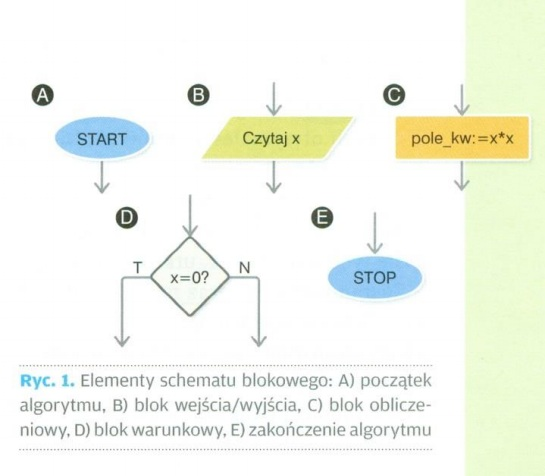
\includegraphics[width=10cm]{rys1}
\end{figure}
\section{Pole kwadratu}
\begin{figure}[ht]
\centering
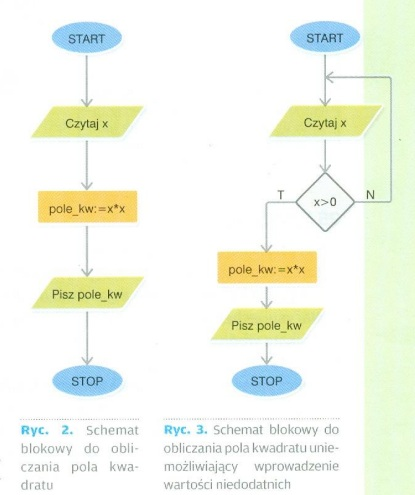
\includegraphics[width=7cm]{rys2}
\end{figure}
\newpage

\section{Czy liczba jest parzysta?}
\begin{figure}[ht]
\centering
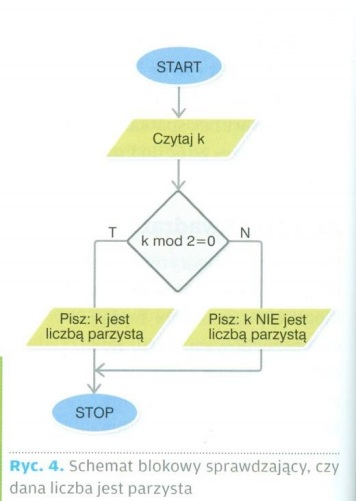
\includegraphics[width=5cm]{rys3}
\end{figure}
\section{Pętle iteracyjne i warunkowe}
\begin{figure}[ht]
\centering
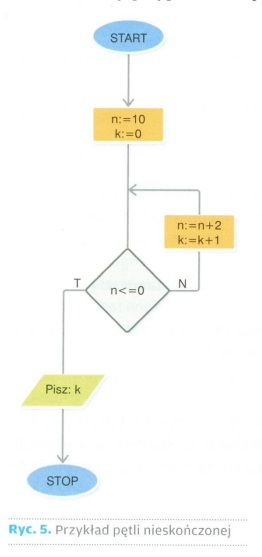
\includegraphics[height=10cm]{rys4}
\end{figure}
\newpage

\section{Suma N Liczb}
\begin{figure}[ht]
\centering
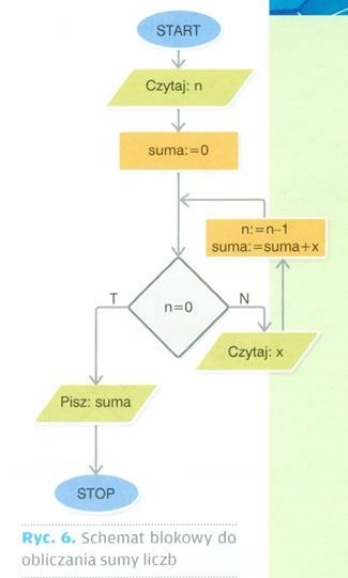
\includegraphics[width=5cm]{rys5}
\end{figure}
\section{Średnia arytmetyczna N Liczb}
\begin{figure}[ht]
\centering
\subfloat{
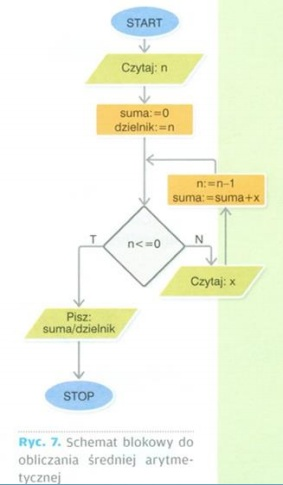
\includegraphics[width=0.35\textwidth]{rys6}}
\quad
\subfloat{
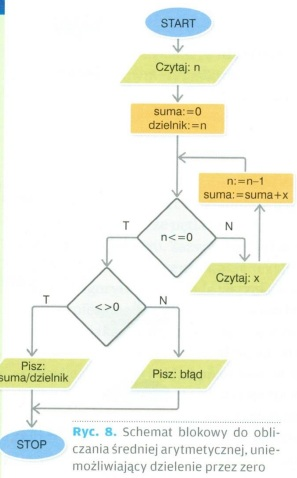
\includegraphics[width=0.35\textwidth]{rys7}}
\end{figure}
\newpage

\section{Suma dowolnie długiego ciągu liczb}
\begin{figure}[ht]
\centering
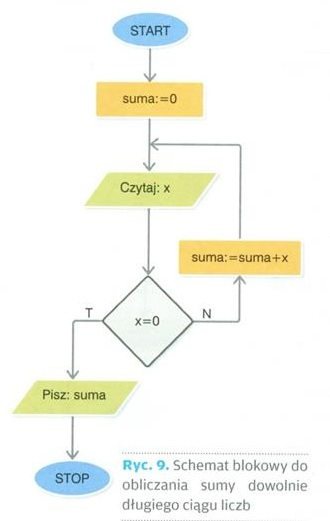
\includegraphics[height=16cm]{rys8}
\end{figure}
\newpage
\section{Wszystkie dzielniki liczby}
\begin{figure}[ht]
\centering
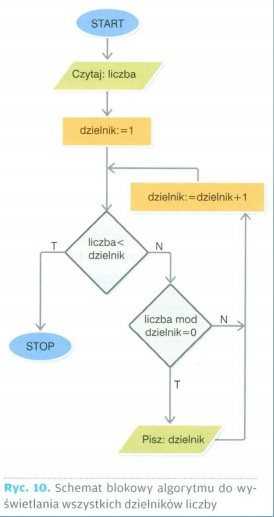
\includegraphics[height=16cm]{rys9}
\end{figure}
\newpage

\section{Sortowanie bąbelkowe}
\begin{wrapfigure}{a}{0.62\textwidth}
\begin{center}
\vspace{-20pt}
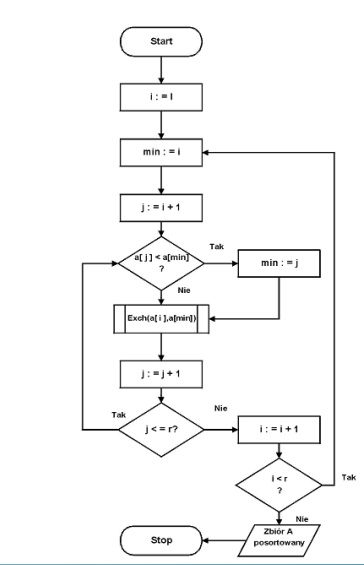
\includegraphics[width=0.6\textwidth]{rys10}
\end{center}
\vspace{-20pt}
\vspace{-10pt}
\end{wrapfigure}
Sortowanie bąbelkowe jest jednym z prostszych w 
implementacji algorytmów sortowania. Swoją nazwę 
zawdzięcza temu, że w przypadku pionowego przedstawienia 
zbioru danych, element najmniejszy(o najmniejszej masie) 
wypływa do góry. Działanie tego algorytmu opiera się na 
porównywaniu każdego elementu z elementem 
następującym po nim i w przypadku stwierdzenia 
nieprawidłowej relacji pomiędzy tymi elementami następuje 
zamiana ich kolejności. 
Wynika to z założenia, że nieposortowany ciąg zawiera, co 
najmniej dwa elementy znajdujące się na nieodpowiednich 
miejscach. Kolejnym krokiem jest sprawdzenie, czy 
poczyniona przez algorytm zmiana kolejności dwóch 
elementów nie wpłynęła na prawidłowość relacji pozostałych 
elementów. Jeżeli zaburzyła tą prawidłowość, zbiór danych 
jest ponownie przeszukiwany w tym samym kierunku. 
Algorytm kończy swoje działanie w przypadku stwierdzenia, 
że wszystkie elementy znajdują się w prawidłowej relacji, czyli 
że nie została wykonana jakakolwiek zamiana kolejności 
elementów. Pesymistyczny koszt takiego algorytmu wynosi 
\begin{math}
n^{2}
\end{math}, gdzie n oznacza ilość elementów do posortowania. 
Algorytm ten jest bardzo wydajny, jeżeli używamy go do 
zbioru danych o bardzo małej ilości elementów, lub też zbiór 
danych jest prawie posortowany (wymaga bardzo małej ilości 
zmian). W przypadku sortowania tablicy posortowanej 
malejąco, algorytm wykona n2
 kroków, jest to wariant 
najbardziej pesymistyczny.
\newpage
\section{Sortowanie szybkie}
\begin{wrapfigure}{b}{0.62\textwidth}
\begin{center}
\vspace{-20pt}
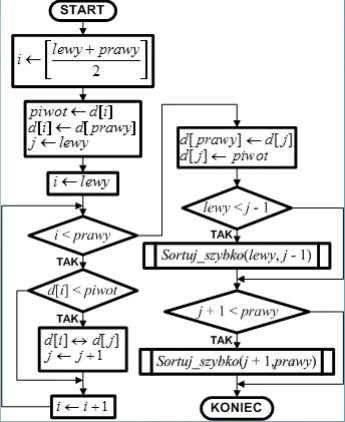
\includegraphics[width=0.6\textwidth]{rys11}
\end{center}
\vspace{-20pt}
\vspace{-10pt}
\end{wrapfigure}
Jest to kolejny z algorytmów sortowania opierający się na 
zasadzie "dziel i zwyciężaj". W algorytmie tym 
wprowadzono pewną dozę prawdopodobieństwa, 
mianowicie. Na początku wybieramy pewien element 
tablicy, tzw. element dzielący, po czym na początek tablicy 
przenosimy wszystkie elementy mniejsze od niego, na 
koniec wszystkie większe, a w powstałe między tymi 
obszarami puste miejsce trafia wybrany element. Potem 
sortujemy osobno początkową i końcową część tablicy. 
Rekursja kończy się, gdy kolejny fragment uzyskany z 
podziału zawiera pojedynczy element, jako że 
jednoelementowa podtablica jest oczywiście posortowana. 
Spójrzmy na jedna rzecz, mianowicie na wagę wyboru 
elementu dzielącego, gdy będziemy wybierać zawsze skrajny 
przypadek, możemy spowodować, że posortowanie już 
posortowanej tablicy będzie zadaniem trudnym. 
Tak więc odrzucimy taki sposób wyboru elementu dzielącego. 
Drugi sposób wykorzystuję już wspomniany przez nas element prawdopodobieństwa. Sposób ten 
opiera się na losowaniu elementu dzielącego, jako jednego z trzech elementów środkowych co w 
sposób zasadniczy sprowadza prawdopodobieństwo zajścia najgorszego przypadku do wartości 
zaniedbywalnie małych. 
Kolejny sposób polega na wstępnym wyborze trzech elementów z rozpatrywanego fragmentu 
tablicy, i użyciu jako elementu dzielącego tego z trzech, którego wartość leży pomiędzy 
wartościami pozostałych dwu. Można również uzupełnić algorytm o poszukiwanie przybliżonej 
mediany.
\newpage
\section{Sortowanie przez scalanie}
\begin{wrapfigure}{c}{0.62\textwidth}
\begin{center}
\vspace{-20pt}
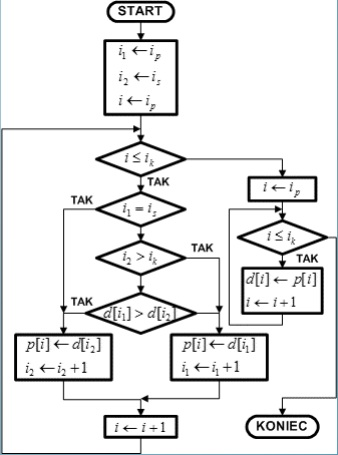
\includegraphics[width=0.6\textwidth]{rys12}
\end{center}
\vspace{-20pt}
\vspace{-10pt}
\end{wrapfigure}
W algorytmie sortowania przez scalanie jest 
wykorzystywana strategia "dziel i zwyciężaj". Strategia 
polega na podzieleniu większego problemu na mniejsze 
takie same problemy a następnie rozwiązywaniu 
mniejszych i scalaniu wyników poszczególnych 
problemów. 
 
 
Algorytm sortowania przez scalanie przedstawia się 
następująco: 
\begin{enumerate}
\item Jeśli ciąg zawiera więcej niż jeden element, to podziel 
go na dwie równe części (lub prawie równe, 
\item jeśli ciąg ma nieparzystą liczbę elementów) posortuj 
pierwszą część stosując ten sam algorytm 
\item Posortuj drugą część stosując ten sam algorytm 
\item Połącz dwa uporządkowane ciągi w jeden ciąg 
uporządkowany 
\end{enumerate}
\newpage
\section{Sortowanie przez wybieranie}
\begin{wrapfigure}{d}{0.62\textwidth}
\begin{center}
\vspace{-20pt}
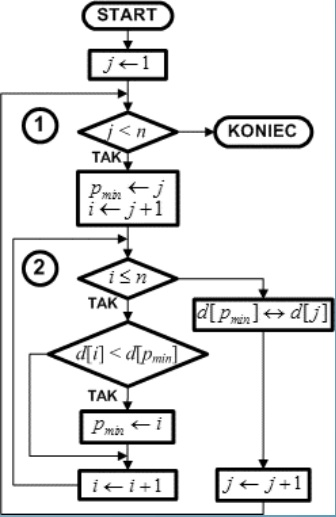
\includegraphics[width=0.6\textwidth]{rys13}
\end{center}
\vspace{-20pt}
\vspace{-10pt}
\end{wrapfigure}
Sortowanie przez wybieranie jest już bardziej wydajnym 
algorytmem sortowania, A niżeli sortowanie bąbelkowe. Idea 
jego działania polega na wybieraniu z podzbioru danych zbioru 
elementu najmniejszego (znajdowania minimum) i zamianie 
jego położenia z początkowym elementem podzbioru. 
Następnie zakres poszukiwania zostaje zawężony do 
podzbioru danych znajdujących się po posortowanych już 
elementach (co krok zbiór będzie mniejszy o 1). W pierwszym 
przeszukiwaniu tym podzbiorem jest naturalnie cały zbiór. 
Koszt tego algorytmu jest zauważalnie mniejszy od 
algorytmów bąbelkowego i sortowania przez wstawianie. 
Wynosi on w pesymistycznym wypadku \begin{math}
\frac{n^{2}-n}{2}
\end{math}, gdzie n 
oznacza ilość elementów do posortowania. Zaletami 
algorytmu sortowania przez wybieranie jest optymalna ilość 
przestawień (n-1); prostota implementacji oraz zadowalająca 
szybkość dla małych wartości n. 
Algorytm przedstawia się następująco:
\begin{enumerate}
\item wyszukaj minimalną wartość z tablicy spośród elementów 
od i+1 do końca tablicy 
\item zamień wartość minimalną, z elementem na pozycji i 
\item przesuń początek zbioru o 1 w przód 
\end{enumerate}
\newpage
\section{Sortowanie przez wstawianie}
\begin{wrapfigure}{e}{0.62\textwidth}
\begin{center}
\vspace{-20pt}
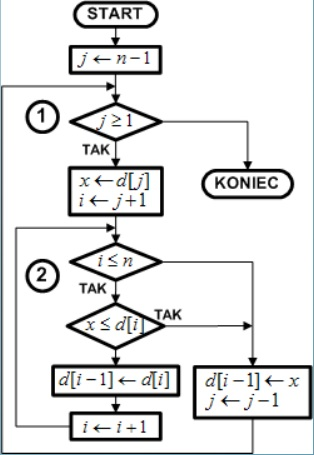
\includegraphics[width=0.6\textwidth]{rys14}
\end{center}
\vspace{-20pt}
\vspace{-10pt}
\end{wrapfigure}
Algorytm ten jest przydatny przy sortowaniu danych 
sukcesywnie napływających. Podobnie jak w przypadku 
algorytmów bąbelkowego i sortowania przez 
wybieranie pesymistyczny koszt działania tego 
algorytmu wynosi \begin{math}
\frac{n^{2}-n}{2}
\end{math}, gdzie n oznacza ilość 
elementów do posortowania. 
Schemat działania algorytmu: 
\begin{enumerate}
\item Utwórz zbiór elementów posortowanych i przenieś 
do niego dowolny element ze zbioru 
nieposortowanego. 
\item Weź dowolny element ze zbioru nieposortowanego. 
\item Wyciągnięty element porównuj z kolejnymi 
elementami zbioru posortowanego póki nie 
napotkasz elementu równego lub elementu 
większego (jeśli chcemy otrzymać ciąg niemalejący) 
lub nie znajdziemy się na początku/końcu zbioru 
uporządkowanego. 
\item Wyciągnięty element wstaw w miejsce gdzie 
skończyłeś porównywać. 
\item Jeśli zbiór elementów nieuporządkowanych jest 
niepusty wróć do punkt 2. 
\end{enumerate}
\end{document}

